\documentclass[11pt, twoside, pdftex]{article}

% This include all the settings that we should use for the document
\newcommand{\PDFTitle}{Altera\textsuperscript{\textregistered} DE10-Lite Computer with Nios~V}
\newcommand{\commonFiles}{../../../common/doc}
\newcommand{\commonFigs}{../../../common/figs}
\newcommand{\sampleProgramsPath}{../../../sample_programs}
\newcommand{\commonPath}{../../../../../Tutorials/Common}
\newcommand{\includesPath}{../../software}
\newcommand{\templatePath}{../../../../../Tutorials/Common}
\input{\templatePath/Docs/defaulttext.tex}
\input{\templatePath/Docs/preamble.tex}

%%%%%%%%%%%%%%%%%%%%%%%%%
% Add title
\newcommand{\doctitle}{DE10-Lite Computer System with Nios\textsuperscript{\textregistered} V}
\newcommand{\dochead}{DE10-Lite Computer System with Nios\textsuperscript{\textregistered} V}
% Usually no need to change these two lines
%\title{\fontfamily{phv}\selectfont{\doctitle} }
%\chead{ \small{\textsc{\bfseries \dochead} } }
% Customizations
\newcommand{\DEBoard}{DE10-Lite}
\newcommand{\systemName}{DE10-Lite Computer}
\newcommand{\systemNameFull}{DE10-Lite Computer with Nios~V}
\newcommand{\systemBuilder}{Platform Designer}
\newcommand{\FPGADeviceFamily}{MAX\textsuperscript{\textregistered} 10}
\newcommand{\processor}{Nios~V}
\newcommand{\BaseAddressOffset}{0}
\newcommand{\baseAddressOffset}{0}
\newcommand{\GIC}{processor}
\newcommand{\VideoOutDevice}{VGA}
\newcommand{\PixelBufferInfo}{160120_16}
\newcommand{\ExpansionPortA}{JP1}
\newcommand{\ExpansionPortB}{JP2}
\newcommand{\processorStyle}{defaultNiosVStyle}
\newcommand{\processorLower}{niosv}

%%\newcommand{\red}[1]{{\color{red}\sf{#1}}}
%%%%%%%%%%%%%%%%%%%%%%%%%

%%%%%%%%%%%%%%%%%%
%%% DOCUMENT START
%\begin{document}
\begin{document}
\begin{table}
    \centering
    \begin{tabular}{p{5cm}p{4cm}}
        % \hspace{-3cm}\includegraphics[width=0.4\textwidth]{\headerlogofilepath{\templatepath/figures}}
        \hspace{-3cm}
        &
        \raisebox{1\height}{\parbox[h]{0.5\textwidth}{\large\fontfamily{phv}\selectfont{\textsf{\doctitle}}}}
    \end{tabular}
    \label{tab:logo}
\end{table}

\colorbox[rgb]{0,0.384,0.816}{\parbox[h]{\textwidth}{\color{white}\textsf{\textit{\textBar}}}}

\thispagestyle{plain}

\section{Introduction}
This document describes a computer system that can be implemented
on the \DEBoard~development and education board, which
is described in the \texttt{Teaching and Projects Boards} 
section of the {\small \href{https://www.fpgacademy.org/boards.html} {FPGAcademy.org}} website. 
This system, called the {\it \systemNameFull}, is intended for use in
experiments on computer organization and embedded
systems. 



To support such experiments, the computer system contains
an embedded processor, memory, basic I/O devices like switches and lights,
video output, and various other I/O peripherals. 
The FPGA programming file that implements this system, as well as its 
design source files, can be obtained from its 
\href{https://github.com/fpgacademy/Design_Examples/tree/main/Computer_Systems} {GitHub repository}.

\section{\systemNameFull~Contents}

A block diagram that displays the components available in the {\it \systemNameFull}~is shown 
in Figure~\ref{fig:block_diagram}. The \processor\textsuperscript{\textregistered} 
processor and ports connected to its peripherals are implemented in the {\it Field-Programmable Gate Array}
(FPGA) in Altera's \FPGADeviceFamily~chip.  The peripheral ports include: memory, timer modules, 
video-out, analog-to-digital, an accelerometer, an expansion port, and parallel ports connected to switches 
and lights.  

\begin{figure}[h!]
   \begin{center}
        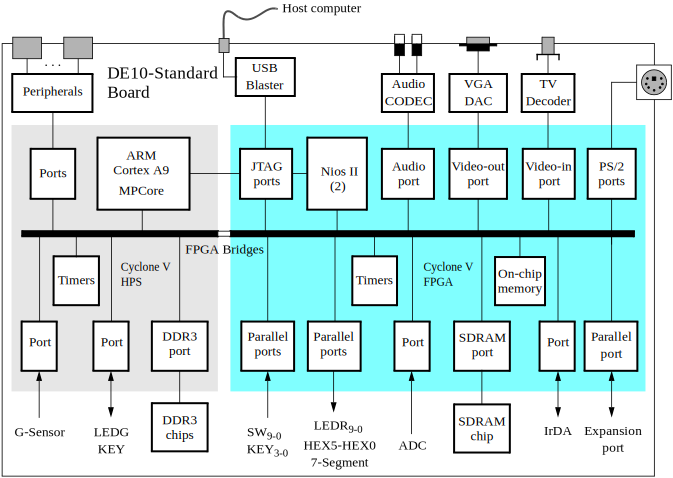
\includegraphics[height=.45\paperheight]{figures/fig_block_diagram.pdf}
   \end{center}
   \caption{Block diagram of the {\it \systemNameFull}.}
	\label{fig:block_diagram}
\end{figure}

\subsection{Getting Started with the \systemNameFull}

To make use of the {\it \systemNameFull} you need to be able to assemble software programs 
for the {\processor} processor and then execute these programs in the computer system. There are 
two main approaches for getting started: using a simulation of the computer system, or
using an FPGA board that implements the computer system in hardware.

\subsubsection {Using the CPUlator Simulator}

The {\it CPUlator} is a powerful and easy-to-use functional simulator that runs inside a
web browser. It simulates the behavior of a whole computer system, including the
processor, memory, and many types of I/O devices. The CPUlator simulator supports computer systems
based on a variety of different processors, including {\it \processor}. 

The CPUlator user interface displays all of the information that a programmer needs to
develop and debug software code running on the {\it \systemNameFull}. CPUlator allows you
to select a specific processor and computer system; to simulate the {\it \systemNameFull}, we would select
the system named \texttt{RISC-V RV32 DE1-SoC}. This selection chooses a computer system that is slightly
different from the {\it \systemNameFull}, but with all of its most important features. The CPUlator shows 
(and allows you to edit) the values in the processor general-purpose and control registers, as well as the 
contents of memories in the computer system and the values of memory-mapped I/O device 
registers. The CPUlator allows software code, written either in assembly language or the 
C language, to be entered into the simulator, assembled to produce machine code, loaded 
into memory, and then executed. The user can set breakpoints in the machine code, 
single-step instructions, and perform any of the usual operations that are supported in 
typical debugging environments. A screen capture of the CPUlator user interface is shown 
in Figure~\ref{fig:CPUlator}. It displays the processor registers on the 
left-hand side (by default) of the screen,
the program code in the middle, and graphical representations of I/O devices on the 
right-hand side.

\begin{figure}[h!]
   \begin{center}
        \includegraphics[scale=.66]{figures/CPUlator.pdf}
   \end{center}
   \caption{The CPUlator.}
	\label{fig:CPUlator}
\end{figure}

\subsubsection {Using an FPGA Hardware Board}

The {\it \systemNameFull} can be implemented using a {\DEBoard} hardware
board.  An easy way to begin working with this hardware system is to make use of the tools
provided with the GNU Project Debugger (GDB) for Nios~V. Detailed instructions for setting up 
these GDB tools are given in the tutorial called {\it Using GDB with Nios V}, which is available
as part of the \texttt{Computer Organization and System Design} tutorials in the 
{\small \href{https://www.fpgacademy.org/tutorials.html} {FPGAcademy.org}} website.

\subsection{Nios\textsuperscript{\textregistered} V Processor}
\label{sec:niosV}
The Altera Nios\textsuperscript{\textregistered}~V processor 
is an implementation of the 32-bit RISC-V processor architecture. Three versions of 
Nios~V exist, each with different features and capabilities.  Documentation for these 
three versions, designated as {\it compact} (Nios~V/c), {\it microcontroller} (Nios~V/m),
and {\it general purpose} (Nios~V/g), can be found by searching on the Internet for keywords 
such as \texttt{Nios~V versions}. The {\it \systemNameFull}~includes 
the Nios~V/g version. An overview of the \processor~processor can be found in the 
document {\it Introduction to \processor}, which is available in the 
Tutorials tab of the 
{\small \href{https://www.fpgacademy.org/tutorials.html} {FPGAcademy.org}} website.

\subsubsection{Nios~V Machine Timer and Software Interrupt Registers}
\label{sec:mtimer}
Nios~V includes a 64-bit internal timer that can be used by application programmers. 
The timer is reset to 0 when the {\DEBoard} board is powered on, and then monotonically
increases at the system clock rate, which is 100~MHz. The timer is accessible via two 
memory-mapped registers, 
called {\it mtime} (machine time) and {\it mtimecmp} (machine time compare). The 
{\it mtime} register provides the current timer value, and the {\it mtimecmp} register 
can be used to cause a timer interrupt. A Nios~V timer interrupt will be pending whenever 
the value of {\it mtime} reaches or exceeds the value of {\it mtimecmp}. Interrupts are 
discussed in Section~\ref{sec:exceptions}.

Since they are 64-bits wide, both {\it mtime} and {\it mtimecmp} comprise two 32-bit 
memory-mapped registers, one for the {\it low} word and the other for the {\it high} word. 
Nios~V also contains a memory-mapped register called {\it msip} (machine software interrupt
pending), which can be used by an application programmer to cause a {\it software interrupt}.

The {\it mtime}, {\it mtimecmp} and {\it msip} memory-mapped registers are 
are illustrated in Figure~\ref{fig:mm_control}, which gives the assigned address of each 
register in the {\it \systemNameFull}.

\begin{figure}[h]
   \begin{center}
      \includegraphics[scale=.9]{figures/mm_control_registers.pdf}
   \caption{Nios~V memory-mapped registers.} 
	 \label{fig:mm_control}
	 \end{center}
\end{figure}

\subsection{Memory Components}

The {\it \systemNameFull} has an SDRAM port, as well as two memory modules 
implemented using the on-chip memory inside the FPGA. These memories are described below.

\subsubsection{SDRAM}
An SDRAM Controller in the FPGA provides an interface to the 64 MB synchronous dynamic RAM (SDRAM) 
on the \DEBoard~board, which is organized as 32M {\sf x} 16 bits. It is
accessible by the \processor~processor using word (32-bit), halfword (16-bit), or byte
operations, and is mapped to the address space {\sf 0x\baseAddressOffset 0000000} to {\sf 0x\baseAddressOffset 3FFFFFF}.




\subsubsection{On-Chip Memory}
A 64 KB memory is implemented inside the FPGA, organized as 16K {\sf x} 32 bits. The 
{\processor} processor can access this memory using addresses in the range 
{\sf 0x\BaseAddressOffset 8000000} to {\sf 0x\BaseAddressOffset 800FFFF}. This
memory is used as a pixel buffer for the video-out port.

\subsubsection{On-Chip Memory Character Buffer}
An 8 KB memory is implemented inside the FPGA for use as a character buffer for the video-out
port, which is described in Section~\ref{sec:video_out}.
The character buffer memory is organized as 8K {\sf x} 8 bits, and spans the {\processor}
address range {\sf 0x\baseAddressOffset 9000000} to {\sf 0x\baseAddressOffset 9001FFF}.



\subsection{Parallel Ports}
There are several parallel ports implemented in the FPGA that support input, output, and
bidirectional transfers of data between the \processor~processor and I/O peripherals. As 
illustrated in Figure~\ref{fig:parallel_port}, each parallel port is assigned a {\it Base}
address and contains up to four 32-bit registers. Ports that have output capability include a
writable {\it Data} register, and ports with input capability have a readable {\it
Data} register. Bidirectional parallel ports also include a {\it Direction} register that 
has the same bit-width as the {\it Data} register. Each bit in the {\it Data} register can be
configured as an input by setting the corresponding bit in the {\it Direction} register to 0,
or as an output by setting this bit position to~1. The {\it Direction} register is assigned the
address {\it Base} + 4.

\begin{figure}[h!]
   \begin{center}
       \includegraphics{../../../common/figs/FPGA_PP.pdf}
   \end{center}
   \caption{Parallel port registers in the {\it \systemNameFull}.}
	\label{fig:parallel_port}
\end{figure}

Some of the parallel ports have registers at addresses 
{\it Base} + 8 and {\it Base} + C, as indicated in Figure~\ref{fig:parallel_port}. These
registers are discussed in Section \ref{sec:exceptions}.



\subsubsection{Red LED Parallel Port}

The red lights {\it LEDR}$_{9-0}$ on the \DEBoard~board
are driven by an output parallel port, as illustrated in Figure \ref{fig:LED_port}. The port
contains a 10-bit {\it Data} register, which has the
address {\sf 0xFF200000}.  This register can be written or read by the processor using word 
accesses, and the upper bits not used in the registers are ignored.

\begin{figure}[h!]
   \begin{center}
       \includegraphics{../../../common/figs/FPGA_PP_Red_LEDs_10.pdf}
   \end{center}
   \caption{Output parallel port for {\it LEDR}.}
	\label{fig:LED_port}
\end{figure}



\subsubsection{7-Segment Displays Parallel Port}

There are two parallel ports connected to the 7-segment displays on the \DEBoard~board, each of
which comprises a 32-bit write-only {\it Data} register. As indicated in 
Figure \ref{fig:hex_segment_port}, the register at address {\sf 0xFF200020} 
drives digits {\it HEX3} to {\it HEX0}, and the register at 
address {\sf 0xFF200030} drives digits {\it HEX5} and
{\it HEX4}.  Data can be written into these two registers, and read back, by using word operations. 
This data directly controls the segments of each display, according to
the bit locations given in Figure \ref{fig:hex_segment_port}. The locations of segments 
6 to 0 in each seven-segment display on the \DEBoard~board is illustrated on the right side of the
figure.

\begin{figure}[h!]
   \begin{center}
       \includegraphics{../../../common/figs/FPGA_PP_7_Segs_6.pdf}
   \end{center}
   \caption{Bit locations for the 7-segment displays parallel ports.}
	\label{fig:hex_segment_port}
\end{figure}


\subsubsection{Slider Switch Parallel Port}

The {\it SW}$_{9-0}$ slider switches on the \DEBoard~board are connected to an input parallel
port.  As illustrated in Figure~\ref{fig:slider_port}, this port 
comprises a 10-bit read-only {\it Data} register, which is mapped to address {\sf 0xFF200040}.

\begin{figure}[h!]
   \begin{center}
       \includegraphics{../../../common/figs/FPGA_PP_Switches_10.pdf}
   \end{center}
   \caption{{\it Data} register in the slider switch parallel port.}
	\label{fig:slider_port}
\end{figure}


\subsubsection{Pushbutton Key Parallel Port}

The parallel port connected to the {\it KEY}$_{1-0}$ 
pushbutton switches on the \DEBoard~board comprises three 2-bit
registers, as shown in Figure \ref{fig:pushbutton_port}. These registers have 
the base address {\sf 0xFF200050} and can be accessed using word operations. 
The read-only {\it Data} register provides the values of the switches {\it KEY}$_{1-0}$. 
The other two registers shown in Figure \ref{fig:pushbutton_port}, at addresses
{\sf 0xFF200058} and {\sf 0xFF20005C}, are discussed in Section \ref{sec:exceptions}.
~\\
~\\
\begin{figure}[h!]
   \begin{center}
       \includegraphics{../../../common/figs/FPGA_PP_Keys_2.pdf}
   \end{center}
   \caption{Registers used in the pushbutton parallel port.}
	\label{fig:pushbutton_port}
\end{figure}
\subsubsection{Expansion Parallel Port}

The \systemName~includes one bidirectional parallel port that is connected to the
{\it \ExpansionPortA} expansion header on the \DEBoard~board. This parallel port
includes the four 32-bit registers that were described previously for 
Figure~\ref{fig:parallel_port}. The base address of this port is {\sf 0xFF200060}.
Figure \ref{fig:expansion_port}$a$ gives a diagram of 
the {\it JP1} expansion connector on the \DEBoard~board, and shows how the respective parallel port {\it Data} register bits, 
$D_{31-0}$, are assigned to the pins on the connector. The figure shows that bit $D_0$ of
the parallel port is assigned to the pin at the top right corner of the
connector, bit $D_1$ is assigned below this, and so on. Note that some of the pins on
{\it \ExpansionPortA} are not usable as input/output connections, and are 
therefore not used by the parallel ports. Also, only 32 of the 36 data pins that appear on
each connector can be used.

\begin{figure}[h!]
   \begin{center}
       \includegraphics{../../../common/figs/FPGA_PP_Expansion_and_Arduino.pdf}
   \end{center}
   \caption{Assignment of parallel port bits to pins.}
	\label{fig:expansion_port}
\end{figure}

\subsubsection{Arduino* Expansion Parallel Port}

The \systemName~includes a bidirectional parallel port that is connected to the
Arduino* Uno R3 expansion header {\it JP2}/{\it JP3} on 
the \DEBoard~board.  This parallel port has the base address {\sf 0xFF200100} and includes the 
four 32-bit registers that were described previously for Figure~\ref{fig:parallel_port}.
The mapping of data bits from this port to the pins on {\it JP2} and {\it JP3} 
is illustrated in part~$b$ of Figure~\ref{fig:expansion_port}.
This mapping connects data bit 0 in the {\it Data} register 
to the signal {\it Arduino\_IO0}, data bit 1 to {\it Arduino\_IO1}, and so on.  

The \systemName~also includes a one-bit output parallel port that is connected to the
{\it Arduino\_Reset\_n} pin on header {\it JP8} on the \DEBoard~board.  
Data bit 0 of this one-bit output port is connected to pin 3 of {\it JP8}, which is the 
{\it Arduino\_Reset\_n} signal.  The address of this port is {\sf 0xFF200110}.

More details about the Arduino Uno R3 expansion header can be found in the 
\DEBoard~Board User Manual.


\input{\commonFiles/FPGA_PP_Examples.tex}

\subsection{JTAG* Port}
\label{sec:jtag_port}

The JTAG* port implements a communication link between the \DEBoard~board and its host computer.  
This link can be used by the Quartus\textsuperscript{\textregistered} Prime software to transfer FPGA programming files 
into the \DEBoard~board, and by the \productNameMed{}, discussed in 
Section~\ref{sec:monitor_program}.  The JTAG port also
includes a UART, which can be used to transfer character data between the host computer and
programs that are executing on the \processor~processor.
The programming interface 
of the JTAG UART consists of two 32-bit registers, as shown in Figure \ref{fig:jtag_port}. 
The register mapped to address {\sf 0xFF201000} is called the {\it Data}
register and the register mapped to address {\sf 0xFF201004} is called the {\it Control}
register.

\begin{figure}[h!]
   \begin{center}
       \includegraphics{../../../common/figs/FPGA_JTAG_UART.pdf}
   \end{center}
   \caption{JTAG UART registers.}
	\label{fig:jtag_port}
\end{figure}

When character data from the host computer is received by the JTAG UART 
it is stored in a 64-character FIFO.  The number of characters currently stored in this FIFO is
indicated in the field {\it RAVAIL}, which are
bits 31$-$16 of the {\it Data} register.  If the receive FIFO overflows, then
additional
data is lost. When data is present in the receive FIFO, then the value of {\it RAVAIL} will be 
greater than 0 and the value of bit 15, {\it RVALID}, will be 1. Reading the character at
the head of the FIFO, which is provided in bits $7-0$, decrements the value of {\it RAVAIL} 
by one and returns this decremented value as part of the read
operation. If no data is present in the receive FIFO, then {\it RVALID} will 
be set to 0 and the data in bits $7-0$ is undefined.

The JTAG UART also includes a 64-character FIFO that stores data 
waiting to be transmitted to the host computer. 
Character data is loaded into this FIFO by performing a write to bits 7$-$0
of the {\it Data} register in Figure \ref{fig:jtag_port}.  
Note that writing into this register has no effect 
on received data.  The amount of space, {\it WSPACE}, currently available in the transmit FIFO is 
provided in bits 31$-$16 of the {\it Control} register.  If
the transmit FIFO is full, then any characters written to the {\it Data} register will be lost.

Bit 10 in the {\it Control} register, called {\it AC}, has the value 1 if the JTAG UART has been
accessed by the host computer. This bit can be used to check if a working connection to
the host computer has been established. The {\it AC} bit can be cleared to 0 by writing a 1
into it.

The {\it Control} register bits {\it RE}, {\it WE}, {\it RI}, and {\it WI} are described 
in Section \ref{sec:exceptions}.

\subsubsection{Using the JTAG* UART with Assembly Language Code and C Code}

Listings \ref{lst:jtag_uart_s} and \ref{lst:jtag_uart_C} give simple examples of 
assembly language and C code, respectively, that use the JTAG UART. Both versions of the
code perform the same function, which is to first send an ASCII string to the JTAG UART,
and then enter an endless loop. In the loop, the code reads character data that has 
been received by the JTAG UART, and echoes this data back to the UART for transmission. In
the {\it CPUlator} simulator, there is a JTAG window that allows text to be typed and
echoed. If the program is executed by using the \productNameMed{}, then any keyboard character that 
is typed into the {\it Terminal Window} of the Monitor Program will be 
echoed back, causing the character to appear in the {\it Terminal Window}.

The source code files shown in Listings \ref{lst:jtag_uart_s} and \ref{lst:jtag_uart_C}
are made available as part of the  
\productNameMed{}. The files can be found under the heading {\it sample programs}, 
and are identified by the name {\it JTAG UART}.


\subsection{Interval Timers}
\label{sec:interval_port}

The {\it \systemNameFull} includes a timer module implemented in the FPGA that can be used by
the \processor~processor. This timer can be loaded with a preset value, and then counts down to 
zero using a 100-MHz clock. The programming interface 
for the timer includes six 16-bit registers, as illustrated in Figure~\ref{fig:interval_port}.  
The 16-bit register at address {\sf 0xFF202000} provides status information about the timer,
and the register at address {\sf 0xFF202004} allows control settings to be made.  The bit 
fields in these registers are described below:

\begin{itemize}
\item
{\it TO} provides a timeout signal which is set to 1 by the timer when it 
has reached a count value of zero.  The {\it TO} bit can be reset by writing a 0 into it. 
\item 
{\it RUN} is set to 1 by the timer whenever it is currently counting. Write 
operations to the status halfword do not affect the value of the {\it RUN} bit. 

\item 
{\it ITO} is used for generating interrupts, which are discussed in section \ref{sec:exceptions}.

\begin{figure}[h!]
   \begin{center}
       \includegraphics{../../../common/figs/FPGA_Interval_Timers.pdf}
   \end{center}
   \caption{Interval timer registers.}
	\label{fig:interval_port}
\end{figure}

\item
{\it CONT} affects the continuous operation of the timer.  When the timer reaches
a count value of zero it automatically reloads the specified starting count value. If 
{\it CONT} is set to 1, then the timer will continue counting down automatically.
But if {\it CONT} $=0$, then the timer will stop after it has reached a count value of 0. 

\item
({\it START}/{\it STOP}) is used to commence/suspend the operation of the 
timer by writing a 1 into the respective bit.
\end{itemize}

The two 16-bit registers at addresses {\sf 0xFF202008} and {\sf 0xFF20200C}
allow the period of the timer to be changed by
setting the starting count value.  The default setting gives a timer period of 125 msec. 
To achieve this period, the starting value of the count is
100 MHz $\times$ 125 msec $=12.5\times10^6$. It is possible to capture a snapshot of the 
counter value at any time by performing a write to address {\sf 0xFF202010}. This write
operation causes the current 32-bit counter value to be stored into the two 16-bit timer
registers at addresses {\sf 0xFF202010} and {\sf 0xFF202014}. These registers can then be
read to obtain the count value.

A second interval timer, which has an identical interface to the one described above, is also 
available in the FPGA, starting at the base address {\sf 0xFF202020}.


\subsection {Accelerometer}

The \systemName~includes an ADXL345 3-axis digital accelerometer, which can be used to
measure acceleration on the board in three directions. The Accelerometer chip is controlled by the
Accelerometer SPI Mode core, which provides a memory-mapped interface at address {\sf 0xFF204020}
to {\sf 0xFF204021}, as shown in in Figure~\ref{fig:accel_port}.

\begin{figure}[h!]
   \begin{center}
       \includegraphics{../../../common/figs/FPGA_Accelerometer.pdf}
   \end{center}
   \caption{Accelerometer registers.}
	\label{fig:accel_port}
\end{figure}

The ADXL345 chip contains a series of 58 internal registers, {\sf 0x00} to {\sf 0x39}, which are
used to contol the device and store data. To access these registers, the address of the desired
register should be written to the {\it Address} register of the Accelerometer SPI Mode core.
Performing a read or write on the {\it Data} register will then read from or write to the 
requested address on the ADXL345. Commonly used registers of the accelerometer and their address
are listed in Table~\ref{tab:accel_regs}. For a full list of registers, consult the ADXL345 
datasheet.

\begin{table} [h]%
	\begin {center}
		\begin{tabular}{c|c|l}
			{\bf Address} &
			{\bf Register Name} &
			{\bf Description} \\
			\hline
			{\sf 0x32} & 
			{\it DATAX0} & 
			Low-order byte of {\it x}-axis acceleration. 
			\\
			{\sf 0x33} & 
			{\it DATAX1} & 
			High-order byte of {\it x}-axis acceleration.
			\\
			{\sf 0x34} & 
			{\it DATAY0} & 
			Low-order byte of {\it y}-axis acceleration. 
			\\
			{\sf 0x35} & 
			{\it DATAY1} & 
			High-order byte of {\it y}-axis acceleration.
			\\
			{\sf 0x36} & 
			{\it DATAZ0} & 
			Low-order byte of {\it z}-axis acceleration. 
			\\
			{\sf 0x37} & 
			{\it DATAZ1} & 
			High-order byte of {\it z}-axis acceleration.
			\\
		\end{tabular}
	\end{center}
\caption{Commonly used registers in the ADXL345 chip.}
\label{tab:accel_regs}
\end{table}


\newpage
\section{Exceptions and Interrupts}
\label{sec:exceptions}

The reset address of the {\processor} processor in the {\it \systemNameFull} is set to
{\sf 0x00000000}. The address used for the trap handler for all other exceptions and 
interrupts can be set by the programmer (by writing to the {\it mtvec} control register). 
Table \ref{tab:irq} gives the assignment of IRQ numbers to each of the I/O peripherals in 
the system. The rest of this section describes the interrupt behavior associated 
with the Nios V machine timer, the FPGA interval timer, parallel ports, and serial ports.

\begin{table}[h]
    \begin{center}
    \begin{tabular}{l|l}
            \textbf{Device Name} &
            \textbf{IRQ \#}
        \\\hline
            Nios V software interrupt & 3 \\
            Nios V machine timer & 7 \\
            Interval timer & 16 \\
            Second Interval timer & 17 \\
            Pushbutton KEY port & 18 \\
            JTAG port & 24 \\
            JP1 Expansion port & 27 \\
            Arduino JP2/JP3 Expansion port & 29 \\
            Accelerometer & 31 \\
    \end{tabular}
    \caption{Hardware IRQ interrupt assignment for the {\it \systemNameFull}.}
	 \label{tab:irq}
    \end{center}
\end{table}

\subsection{Interrupts from the Nios V Software Interrupts and Machine Timer}
The IRQ numbers for the Nios V software interrupts register and machine timer are not
system dependent and are part of the processor specification. The procedure that can be used
to set up and handle these interrupts is described in the 
document {\it Introduction to \processor}, which is available as part of the 
\texttt{Computer Organization and System Design} tutorials in the 
{\small \href{https://www.fpgacademy.org/tutorials.html} {FPGAcademy.org}} website.

\subsection{Interrupts from the FPGA Interval Timer}

Figure \ref{fig:interval_port}, in Section \ref{sec:interval_port}, shows six registers that
are associated with the interval timer. As we said in Section \ref{sec:interval_port}, the
{\it TO}~bit in the {\it Status} register is set to 1 when the timer reaches a count value of 0.
It is possible to generate an interrupt when this occurs, by using the {\it ITO}~bit in 
the {\it Control} register. Setting the {\it ITO}~bit to 1 causes an interrupt request to 
be sent to the \GIC~whenever {\it TO} becomes 1. After an interrupt occurs, it can be cleared 
by writing any value into the {\it Status} register.



\subsection{Interrupts from Parallel Ports}

Parallel ports were illustrated in Figure~\ref{fig:parallel_port}, which is reproduced 
as Figure~\ref{fig:parallel_port_int}.
As the figure shows, parallel ports that support interrupts include two related registers 
at the addresses {\it Base} + 8 and {\it Base} + C.
The {\it Interruptmask} register, which has the address {\it Base} + 8, specifies whether 
or not an interrupt signal should be sent to the \GIC~when the data present at
an input port changes value.  Setting a bit location in this register to 1 allows 
interrupts to be generated, while setting the bit to 0 prevents interrupts. 
Finally, the parallel port may contain an {\it Edgecapture} register at address
{\it Base} + C.  Each bit in this register has the value 1 if the 
corresponding bit location in the parallel port has changed its value from 0 to 1.
A bit in the {\it Edgecapture} register can be cleared to 0
by writing a 1 into the corresponding bit position, which clears any associated interrupt. 

\begin{figure}[h!]
   \begin{center}
       \includegraphics{../../../common/figs/Interrupts_FPGA_PP.pdf}
   \end{center}
   \caption{Registers used for interrupts from the parallel ports.}
	\label{fig:parallel_port_int}
\end{figure}



\subsubsection{Interrupts from the Pushbutton Keys}

Figure \ref{fig:pushbutton_port}, reproduced as Figure \ref{fig:pushbutton_port_int},
shows the registers associated with the pushbutton parallel port. 
The {\it Interruptmask} register allows processor interrupts to be generated when a key is
pressed.  Each bit in the {\it Edgecapture} register is set to 1 by the parallel port when the
corresponding key is pressed. The processor can read this register
to determine which key has been pressed, in addition to receiving an interrupt request if the
corresponding bit in the {\it Interruptmask} register is set to 1. Writing a 1 into a bit position
in the {\it Edgecapture} register clears the bit to 0 and deasserts the interrupt request.

\begin{figure}[h!]
   \begin{center}
       \includegraphics{../../../common/figs/FPGA_PP_Keys_2.pdf}
   \end{center}
   \caption{Registers used for interrupts from the pushbutton parallel port.}
	\label{fig:pushbutton_port_int}
\end{figure}
\subsection{Interrupts from the JTAG* UART}

Figure \ref{fig:jtag_port}, reproduced as Figure \ref{fig:jtag_port_int}, shows the {\it Data} 
and {\it Control} registers of the JTAG UART. As we said in Section~\ref{sec:jtag_port}, 
{\it RAVAIL} in the {\it Data} register gives the number of characters that 
are stored in the receive 
FIFO, and {\it WSPACE} gives the amount of unused space that is available in the transmit FIFO. 
The {\it RE} and {\it WE} bits in Figure \ref{fig:jtag_port_int}
are used to enable processor interrupts associated with the receive and transmit FIFOs. 
When enabled, interrupts are generated when {\it RAVAIL} for the receive FIFO, 
or {\it WSPACE} for the transmit FIFO, exceeds 7. Pending interrupts are indicated in the 
Control register's {\it RI} and {\it WI} bits, and can be cleared by writing or reading data
to/from the JTAG UART.

\begin{figure}[h!]
   \begin{center}
       \includegraphics{../../../common/figs/FPGA_JTAG_UART.pdf}
   \end{center}
   \caption{Interrupt bits in the JTAG UART registers.}
	\label{fig:jtag_port_int}
\end{figure}




\subsection{Using Interrupts with Assembly Language Code}

An example of assembly language code for the {\it \systemNameFull} that uses interrupts is
shown in Listing \ref{lst:interrupt_example_s}. When this code is executed on the
{\DEBoard} board it first sets up interrupts from three devices: the Nios~V machine timer, 
an FPGA interval timer, and the pushbutton KEY port. The code to initialize these devices
is given in Lines 141 to 175 in Part ($d$) of Listing \ref{lst:interrupt_example_s}. 
Line 24 in Listing \ref{lst:interrupt_example_s}($a$) initializes the stack pointer to
the bottom of the 64~MB SDRAM on the {\DEBoard}, and Lines 25 to 27 initialize the
three interrupting devices. Interrupts are enabled in Lines 30 to 37. First, the address of
the trap handler routine is written into the {\it mtvec} register, and then software
interrupts, machine timer, interval timer, and KEY port interrupts are
enabled by setting bits $b_3$, $b_7$, $b_{16}$ and $b_{18}$, respectively, of the 
machine interrupt enable ({\it mie}) register. 
Finally, interrupts are enabled in Nios~V by setting bit $b_3$ of the {\it mstatus} register.

Next, in Lines 40 to 42 the program makes a software 
interrupt occur, to illustrate how this is done. Finally, the main program loops in
between Lines 51 and 57 while responding to interrupts from the timers and the 
KEY pushbutton port. 

The trap handler is given in Lines 59 to 89. After first saving registers that will be
modified, it reads the value of the {\it mcause} register. Based on this value, the trap
handler calls the appropriate interrupt service routine. 

The interrupt service routine for the software interrupt, in Lines 91 to 97, 
turns on most of the red lights in the \red{LEDR} port, to provide a visual indication of 
its execution. 

The interrupt service routine for the Nios V machine timer, in Lines 99 to 114,
adjusts the {\it mtimecmp} value for the next interrupt, and 
increments a counter variable. The main program displays this counter as a binary number 
on the red lights \red{LEDR}, which will increment for every timer interrupt.

The interrupt service routine for the FPGA interval timer, in Lines 116 to 129,
increments a one-digit decimal counter. The main program displays this counter on the 
7-segment display \red{HEX0}. The counter either increments or decrements,
in the range \red{0} to \red{9}.  When a KEY is pressed, its corresponding 
interrupt service routine, in Lines 131 to 139, reverses the direction of counting on \red{HEX0}. 

The remaining lines of code, in Listing~\ref{lst:interrupt_example_s}($e$),
provide a subroutine for converting decimal digits to 7-segment display codes,
and define the global variables that are used in the program.

\subsection{Using Interrupts with C Code}

An example of C code for the {\it \systemNameFull} that uses interrupts is shown in 
Listing \ref{lst:interrupt_example_C}. This code performs the same operations as
the code in Listing \ref{lst:interrupt_example_s}. Lines 1 to 22 in the code declare some symbols, 
function prototypes, and global variables that are needed in the program. The function
prototype for the {\it handler} subroutine, which is the trap handler in this program, is
assigned the attribute \texttt{interrupt ("machine")}. This attribute instructs the C compiler 
to generate the appropriate assembly-language code for an interrupt handler: it saves and 
restores all registers that could be modified while the interrupt is being handled, and it 
returns to the interrupted program by using the \texttt{mret} instruction. 

The main program declares pointers for accessing I/O devices in Lines 45 to 47. These
pointers are given the \texttt{volatile} keyword, which tells the compiler that the
value of the variables may change at any time, even if not modified in the code where
they are declared (in this case the values may be modified by the interrupt service routines). 
Lines 49 to 51 in the code call subroutines that enable interrupts in the Nios V machine
timer, the FPGA interval timer, and the KEY port. 

Interrupts are enabled in the C code in lines 53 to 66 by inserting assembly-language code 
using the GNU C-compiler's \texttt{\_\_asm\_\_} inline assembly feature. The steps performed by
these lines of code are the same as those in Lines 29 to 37 of 
Listing~\ref{lst:interrupt_example_s}.

Inline assembly-language code is also used in the {\it handler} routine, in Line 84 in 
Part ($b$) of Listing~\ref{lst:interrupt_example_C}, to read the Nios~V {\it mcause} register.
The handler then calls the appropriate interrupt service routine. As mentioned above, the
{\it handler} saves and restores all temporary registers, and returns to the main program 
using the \texttt{mret} instruction, because the
handler is declared with the \texttt{interrupt ("machine")} attribute.

% Section: Media Components
\section{Media Components}
\label{sec:multi}

This section describes the video-out and Analog-to-Digital (ADC) ports,
as well as floating point support.

\subsection{Video-out Port}
\label{sec:video_out}

The {\it \systemNameFull} includes a video-out port connected to the on-board
\VideoOutDevice~controller that can be connected to a standard
\VideoOutDevice~monitor. The video-out port support a screen resolution
of 640 $\times$ 480. The image that is displayed by the video-out port is
derived from two sources: a {\it pixel} buffer, and a {\it character} buffer.

\input{\commonFiles/Media_FPGA_Pixel_Buffer_\PixelBufferInfo.tex}
\input{\commonFiles/Media_FPGA_Double_Buffering_Lite.tex}
\subsubsection{Character Buffer}

The character buffer for the video-out port is stored in on-chip memory in the FPGA
on the \DEBoard~board. As illustrated in Figure \ref{fig:chars}$a$, the buffer provides 
a resolution of 80 $\times$ 60 characters, where each character occupies an 8 $\times$ 8
block of pixels on the screen. Characters are stored in each of the locations shown in
Figure \ref{fig:chars}$a$ using their ASCII codes; when these character codes are 
displayed on the monitor, the character buffer automatically generates the
corresponding pattern of pixels for each character using a built-in font. 
Part $b$ of Figure \ref{fig:chars} shows that characters are addressed in the memory by 
using the combination of a {\it base} address, which has the value 
{\sf 0x\baseAddressOffset 9000000}, and an {\it x,y}
offset. Using this scheme, the character at location 0,0 has the address
{\sf 0x\baseAddressOffset 9000000}, 
the character 1,0 has the address {\it base} $+$ (000000 0000001)$_2$ = {\sf 0x\baseAddressOffset 9000001}, 
the character 0,1 has the address {\it base} $+$ (000001 0000000)$_2$ = {\sf 0x\baseAddressOffset 9000080}, and 
the character at location 79,59 has the address {\it base} $+$ (111011 1001111)$_2$ = 
{\sf 0x\baseAddressOffset 9001DCF}. 

\begin{figure}[h!]
   \begin{center}
       \includegraphics{../../../common/figs/Media_FPGA_Video_Chars.pdf}
   \end{center}
   \caption{Character buffer coordinates and addresses.}
	\label{fig:chars}
\end{figure}

\subsubsection{Using the Video-out Port with C code}

A fragment of C code that uses the pixel and character buffers is shown in 
Listing \ref{lst:video_C}.  The first {\bf for} loop in the figure draws a rectangle in 
the pixel buffer using the color {\it pixel\_color}. The rectangle is drawn using the
coordinates $x_1, y_1$ and $x_2, y_2$.  The second {\bf while} loop in the 
figure writes a null-terminated character
string pointed to by the variable {\it text\_ptr} into the character buffer at the
coordinates {\it x}, {\it y}.






\subsection{Analog-to-Digital Conversion Port}

\label{sec:ADC_port}

The Analog-to-Digital Conversion (ADC) Port provides access to six channels of 12-bit
analog-to-digital conversion on the \DEBoard~board. As illustrated in
Figure~\ref{fig:ADC_port}, the ADC port comprises eight 12-bit registers starting at the
base address {\sf 0xFF204000}. Note that channels 6 and 7 are not used. 
The first two registers have dual purposes, acting as both
data and control registers.  By default, the ADC port updates the A-to-D conversion
results for all ports only when instructed to do so. Writing to the control register at 
address {\sf 0xFF204000} causes this update to occur. Reading from the register at address
{\sf 0xFF204000} provides the conversion data for channel 0. Reading from the other seven
registers provides the conversion data for the corresponding channels. It is also
possible to have the ADC port continually request A-to-D conversion data for all channels.
This is done by writing the value 1 to the control register at address {\sf 0xFF204004}.
The {\it R} bit of each channel register in Figure~\ref{fig:ADC_port} is used in Auto-update mode.
{\it R} is set to 1 when its corresponding channel is refreshed and set to 0 when the channel is read.

\begin{figure}[h!]
   \begin{center}
       \includegraphics{../../../common/figs/Media_FPGA_ADC.pdf}
   \end{center}
   \caption{ADC port registers.}
	\label{fig:ADC_port}
\end{figure}

Figure~\ref{fig:ADC_conn} shows the connector, which is called {\it JP8},
on the \DEBoard~board that is used with the
ADC port. Note that this connector is also used to supply the analog signals that are
part of the Arduino Uno R3 header, meaning that these pins are being shared for these two purposes. 
Analog signals in the range of 0 V to the $V_{CC5}$ power-supply voltage can be 
connected to the pins for channels 0 to 5. Channels 6 and 7 are not connected. 

\begin{figure}[h!]
   \begin{center}
       \includegraphics{../../../common/figs/Media_FPGA_ADC_Conn_Lite.pdf}
   \end{center}
   \caption{ADC connector.}
	\label{fig:ADC_conn}
\end{figure}




\subsection{Floating-point Hardware}
\label{sec:fp}

The Nios~V/g processor in the includes hardware support for
floating-point addition, subtraction, multiplication, and division. To use this support in
a C program, variables must be declared with the type {\it float}. A simple example of 
such code is given in Listing~\ref{lst:fp}. When this code is compiled, it may be necessary 
to pass special argument to the C compiler to instruct it to 
use the floating-point hardware support.

% Section: Modifying the System
\section{Modifying the \systemNameFull}

It is possible to modify the {\it \systemNameFull} 
by using Altera's Quartus\textsuperscript{\textregistered} Prime software
and {\systemBuilder} tool. Instructions for using this software are
provided as part of the
\texttt{Computer Organization and System Design} tutorials on the 
{\small \href{https://www.fpgacademy.org/tutorials.html} {FPGAcademy.org}} website.
To modify the system it is first necessary to make an editable copy of the 
{\it \systemNameFull}. The files for this system are available in its
\href{https://github.com/fpgacademy/Design_Examples/tree/main/Computer_Systems} 
{GitHub repository}.

Locate these files, copy them to a working directory, and then 
use the Quartus Prime and {\systemBuilder} software to make any desired changes.

Table \ref{tab:sopcnames} lists the names of the {\systemBuilder} IP cores that are used 
in this system. When the {\it \systemNameFull} design files are opened in the Quartus 
Prime software, these cores can be examined using the {\systemBuilder} System Integration 
tool.  Each core has a number of settings that are selectable in the {\systemBuilder} 
System Integration tool, and includes a datasheet that provides detailed documentation.

The steps needed to modify the system are:

\begin{enumerate}
\item Make of copy of the design source files for the {\it \systemNameFull} from the its 
GitHub repository. 
\item Open the top-level project file (*.{\it qpf}) in the Quartus Prime software
\item Open the {\systemBuilder} System Integration tool in the Quartus Prime software, and 
modify the system as desired
\item Generate the modified system by using the {\systemBuilder} System Integration tool
\item It may be necessary to modify the Verilog code in the top-level module of the project, 
if any I/O peripherals have been added or removed from the system
\item Compile the project in the Quartus Prime software
\item Download the modified system into the \DEBoard~board
\end{enumerate}

Note: to compile and use a new version of the {\it \systemNameFull} it may be necessary to
request a license from Altera that allows you to create circuit that includes 
the {\processor} processor.


\begin{table}[h]
    \begin{center}
    \begin{tabular}{l|l}
            \textbf{I/O Peripheral}
            & \textbf{Qsys Core}
        \\\hline
            \rule{0in}{0.2in}SDRAM
            & SDRAM Controller
        \\
            On-chip memory character buffer
				& Character Buffer for VGA Display
        \\
            Red LED parallel port
				& Parallel Port
        \\
            7-segment displays parallel port
				& Parallel Port
        \\
            Expansion parallel ports
				& Parallel Port
        \\
            Slider switch parallel port
				& Parallel Port
        \\
            Pushbutton parallel port
				& Parallel Port
        \\
            JTAG port
				& JTAG UART
        \\
            Interval timer
				& Interval timer 
        \\
            System ID
				& System ID Peripheral
        \\
            Video port
				& Pixel Buffer DMA Controller
        \\
    \end{tabular}
    \caption{{\systemBuilder} cores used in the {\it \systemNameFull}.}
    \label{tab:sopcnames}
    \end{center}
\end{table}
\clearpage

% Section: Making the System the Default Configuration
\section{Making the System the Default Configuration}
\label{sec:systempof}

The {\it \systemNameFull} can be loaded into the nonvolatile FPGA configuration memory on the
\DEBoard~board, so that it becomes the default system whenever the board is powered on.
Instructions for configuring the \DEBoard~board in this manner can be found in the tutorial
{\it Introduction to the Quartus Prime Software}, which is available as part of the
\texttt{Digital Logic Hardware Design} tutorials in the 
{\small \href{https://www.fpgacademy.org/tutorials.html} {FPGAcademy.org}} website.




\section{Memory Layout}

\noindent
Table \ref{tab:memorylayout} summarizes the memory map used in the \systemName.
~\\
~\\

\begin{table}[h]
    \begin{center}
    \begin{tabular}{c|c|l}
            \textbf{Base Address}
            & \textbf{End Address}
            & \textbf{I/O Peripheral}
				\\\hline\vspace{-3mm}\\
            0x00000000
            & 0x03FFFFFF
            & SDRAM
        \\
            0x08000000
            & 0x0803FFFF
            & FPGA On-chip Memory
        \\
            0x09000000
            & 0x09001FFF
            & FPGA On-chip Memory Character Buffer
        \\
            0xFF200000
            & 0xFF20000F
            & Red LEDs
        \\
            0xFF200020
            & 0xFF20002F
            & 7-segment HEX3$-$HEX0 Displays
        \\
            0xFF200030
            & 0xFF20003F
            & 7-segment HEX5$-$HEX4 Displays

        \\
            0xFF200040
            & 0xFF20004F
            & Slider Switches
        \\
            0xFF200050
            & 0xFF20005F
            & Pushbutton KEYs
        \\
            0xFF200060
            & 0xFF20006F
            & JP1 Expansion
        \\
            0xFF200070
            & 0xFF20007F
            & JP2/JP3 Arduino\_GPIO
        \\
            0xFF200110
            & 0xFF20011F
            & JP8 Arduino\_Reset\_N
        \\
            0xFF201000
            & 0xFF201007
            & JTAG UART
        \\
            0xFF202000
            & 0xFF20201F
            & Interval Timer
        \\
            0xFF202020
            & 0xFF20202F
            & Second Interval Timer
        \\
            0xFF202100
            & 0xFF202114
            & Nios V Machine Timer and Software Interrupts Registers
        \\
            0xFF203020
            & 0xFF20302F
            & Pixel Buffer Control
        \\
            0xFF203030
            & 0xFF203037
            & Character Buffer Control
        \\
            0xFF204000
            & 0xFF20401F
            & ADC
         \\
            0xFF204020
            & 0xFF204021
            & Accelerometer
        \\
        \\
    \end{tabular}
    \caption{Memory layout used in the \systemName.}
    \label{tab:memorylayout}
    \end{center}
\end{table}

% Section: AMP Integration
% \newpage
\section{\productNameMed{} Integration} 
\label{sec:monitor_program}

As we mentioned earlier, the {\it \systemNameFull} system, and the sample programs described
in this document, are made available as part of the \productNameMed{}. Figures
\ref{fig:monitor_project} to
\ref{fig:monitor_last} show a series of windows that are used in the Monitor 
Program to create a new project.
In the first screen, shown in Figure \ref{fig:monitor_project}, the user specifies a 
file system folder where the
project will be stored, gives the project a name, and specifies the type of processor that
is being used. Pressing {\sf Next} opens the window
in Figure \ref{fig:monitor_system}. Here, the user can select the {\it \systemNameFull} 
as a pre-designed system.
The Monitor Program then fills in the relevant information in the {\it System details} box,
which includes the appropriate system info and FPGA configuration files, and preloader.
The first of these files specifies to the Monitor Program information about the components 
that are available in the {\it \systemNameFull}, such as the type of processor and memory 
components, and the address map. The second file is an FPGA programming bitstream for 
the {\it \systemNameFull}, which can downloaded by the Monitor Program into the \DEBoard~board. 
Any system which contains a Hard Processor System (HPS) component must also specify the preloader to be
run immediately following the circuit being downloaded. This preloader is used to configure the components
within the HPS with the setting required for the specific board.
~\\
~\\
\begin{figure}[h!]
	\centering
	\includegraphics[scale=0.65]{figures/fig_monitor_project.png}
	\caption{Specifying the project folder and project name.}
	\label{fig:monitor_project}
\end{figure}

\clearpage
\newpage
Pressing {\sf Next} again opens the window in Figure \ref{fig:monitor_samples}. Here the
user selects the type of program that will be used, such as Assembly language, or C. Then,
the check box shown in the figure can be used to display the list of sample programs for
the {\it \systemNameFull} that are described in this document. When a sample program
is selected in this list, its source files, and other settings, can be copied into the 
project folder in subsequent screens of the Monitor Program.

Figure \ref{fig:monitor_last} gives the final screen that is 
used to create a new project in the Monitor Program. This screen shows the default addresses of 
compiler and linker sections that will be used for the assembly language or C program 
associated with the Monitor Program project.  In the figure, the drop-down menu called 
{\it Linker Section Presets} has been set to {\sf Exceptions}. With this setting the 
Monitor Program uses specific compiler and linker sections for the selected processor.
For the \processor processor, these sections are for reset and
trap handler, and another section for the main program, called .{\it text}. For the
A9 processor, it has a section for the exception table, 
called .{\it vectors}, and another section
for the main program, called .{\it text}. It also shows the initial value used to set the main 
stack pointer for C programs, which is the starting address of the .{\it stack} section.
~\\
~\\
\begin{figure}[h!]
	\centering
	\includegraphics[scale=0.60]{figures/fig_monitor_system.png}
	\caption{Specifying the {\systemNameFull}.}
	\label{fig:monitor_system}
\end{figure}

\begin{figure}[h!]
	\centering
	\includegraphics[scale=0.55]{figures/fig_monitor_samples.png}
	\caption{Selecting sample programs.}
	\label{fig:monitor_samples}
\end{figure}

\begin{figure}[h!]
\centering
	\includegraphics[scale=0.55]{figures/fig_monitor_last.png}
	\caption{Setting offsets for .{\it text} and .{\it data}.}
	\label{fig:monitor_last}
\end{figure}


\clearpage

% Appendix
\input{\commonFiles/appendix.tex}
\subsection{Parallel Ports}

\expandparam
\lstinputlisting[style=\processorStyle, caption={An example of \processor~assembly
language code that uses parallel ports.}, captionpos=b, label={lst:getting_started_s},
showlines=true]{\sampleProgramsPath/\processorLower/asm/getting_started/getting_started.s}
\newpage

\lstinputlisting[language=C, caption={An example of C code that uses parallel ports.}, captionpos=b, label={lst:getting_started_C}]{\sampleProgramsPath/\processorLower/c/getting_started/getting_started.c}
\newpage
\subsection{JTAG* UART}

% Assembly Source Code
\expandparam
\lstinputlisting[style=\processorStyle, caption={An example of assembly language code that
uses the JTAG UART (Part $a$).}, captionpos =b, label={lst:jtag_uart_s}, lastline=35,
showlines=true]{\sampleProgramsPath/\processorLower/asm/JTAG_UART/JTAG_UART.s}
\newpage
\expandparam
\lstinputlisting[style=\processorStyle, captionpos=b, firstline=36]{\sampleProgramsPath/\processorLower/asm/JTAG_UART/JTAG_UART.s}
\begin{center}
Listing \ref{lst:jtag_uart_s}. An example of assembly language code that uses the JTAG UART (Part {\it b}).
\end{center}
\newpage

\lstinputlisting[language=C, caption={An example of C code that uses the JTAG UART (Part a).}, captionpos=b, label={lst:jtag_uart_C}]{\sampleProgramsPath/\processorLower/c/JTAG_UART/JTAG_UART.c}
\newpage
\lstinputlisting[language=C, captionpos=b]{\sampleProgramsPath/\processorLower/c/JTAG_UART/main.c}
\begin{center}
Listing \ref{lst:jtag_uart_C}. An example of C code that uses the JTAG UART (Part {\it b}).
\end{center}
\newpage


\subsection{Interrupts}

% Assembly source files

% interrupt example
\begin{center} \begin{minipage}[h]{16.5 cm}
\lstinputlisting[style=defaultNiosVStyle, name=interrupt_example_s, caption={An example of assembly language code
that uses interrupts (Part $a$).}, captionpos=b, label={lst:interrupt_example_s}, lastline=43,
showlines=true, numbers=left]{\sampleProgramsPath/niosv/asm/interrupt_example/interrupt_example.s}
\end{minipage} \end{center}

\newpage
\begin{center} \begin{minipage}[h]{15 cm}
\expandparam
\lstinputlisting[style=\processorStyle, name=interrupt_example_s, firstnumber=last,
captionpos=b, firstline=44, lastline=90, showlines=true,
numbers=left]{\sampleProgramsPath/\processorLower/asm/interrupt_example/interrupt_example.s}
\end{minipage} \end{center}
\begin{center}
Listing \ref{lst:interrupt_example_s}. An example of assembly language code that uses
interrupts (Part {\it b}).
\end{center}

\newpage
\begin{center} \begin{minipage}[h]{15 cm}
\expandparam
\lstinputlisting[style=\processorStyle, name=interrupt_example_s, firstnumber=last,
captionpos=b, firstline=91, lastline=130, showlines=true, 
numbers=left]{\sampleProgramsPath/\processorLower/asm/interrupt_example/interrupt_example.s}
\end{minipage} \end{center}
\begin{center}
Listing \ref{lst:interrupt_example_s}. An example of assembly language code that uses
interrupts (Part {\it c}).
\end{center}

\newpage
\begin{center} \begin{minipage}[h]{16 cm}
\expandparam
\lstinputlisting[style=\processorStyle, name=interrupt_example_s, firstnumber=last,
captionpos=b, firstline=131, lastline=176, showlines=true, numbers=left]{\sampleProgramsPath/\processorLower/asm/interrupt_example/interrupt_example.s}
\end{minipage} \end{center}
\begin{center}
Listing \ref{lst:interrupt_example_s}. An example of assembly language code that uses
interrupts (Part {\it d}).
\end{center}

\newpage
\begin{center} \begin{minipage}[h]{16 cm}
\expandparam
\lstinputlisting[style=\processorStyle, name=interrupt_example_s, firstnumber=last,
captionpos=b, firstline=177, showlines=true, numbers=left]{\sampleProgramsPath/\processorLower/asm/interrupt_example/interrupt_example.s}
\end{minipage} \end{center}
\begin{center}
Listing \ref{lst:interrupt_example_s}. An example of assembly language code that uses
interrupts (Part {\it e}).
\end{center}

\newpage
% C Source Code

\begin{center} \begin{minipage}[h]{16.5 cm}
\lstinputlisting[language=C, caption={An example of C code that uses interrupts (Part $a$).},
captionpos=b, label={lst:interrupt_example_C}, numbers=left, lastline=48, showlines=true]{\sampleProgramsPath/niosv/c/interrupt_example/interrupt_example.c}
\end{minipage} \end{center}
\newpage

\begin{center} \begin{minipage}[h]{15 cm}
\lstinputlisting[language=C, numbers=left, firstnumber=last, firstline=49, lastline=95,
showlines=true]{\sampleProgramsPath/niosv/c/interrupt_example/interrupt_example.c}
\end{minipage} \end{center}
\begin{center}
Listing \ref{lst:interrupt_example_C}. An example of C code that uses interrupts (Part {\it b}).
\end{center}
\newpage

\begin{center} \begin{minipage}[h]{15 cm}
\lstinputlisting[language=C, numbers=left, firstnumber=last, firstline=96, lastline=136,
showlines=true]{\sampleProgramsPath/niosv/c/interrupt_example/interrupt_example.c}
\end{minipage} \end{center}
\begin{center}
Listing \ref{lst:interrupt_example_C}. An example of C code that uses interrupts (Part {\it c}).
\end{center}
\newpage

\begin{center} \begin{minipage}[h]{15 cm}
\lstinputlisting[language=C, numbers=left, firstnumber=last, firstline=137,
showlines=true]{\sampleProgramsPath/niosv/c/interrupt_example/interrupt_example.c}
\end{minipage} \end{center}
\begin{center}
Listing \ref{lst:interrupt_example_C}. An example of C code that uses interrupts (Part {\it d}).
\end{center}
\newpage

\subsection{Video Out}

\lstinputlisting[language=C, label={lst:video_C}, caption={An example of code that uses the video-out port.}, captionpos=b]
{\sampleProgramsPath/\processorLower/c/video/video.c}
\newpage

\subsection{Floating Point}

\lstinputlisting[language=C, label={lst:fp}, caption={An example of code that uses floating-point variables.}, captionpos=b]{\sampleProgramsPath/nios2/c/floating/floating.c}
\newpage
\subsection{Include Files}

% Assembly source files

\begin{center} \begin{minipage}[h]{16.5 cm}
\lstinputlisting[style=defaultNiosVStyle, name=interrupt_example_s, caption={The
{\it address\_map\_niosv.s} include file.}, captionpos=b, label={lst:address_map_niosv_s}, 
showlines=true]{\includesPath/address_map_niosv.s}
\end{minipage} \end{center}

\newpage
% C Source Code

\begin{center} \begin{minipage}[h]{16.5 cm}
\lstinputlisting[language=C, caption={The {\it address\_map\_niosv.h} include file.},
captionpos=b, label={lst:address_map_niosv_h},
showlines=true]{\includesPath/address_map_niosv.h}
\end{minipage} \end{center}

\newpage


\input{\templatePath/Docs/copyright.tex}

\end{document}

